 \documentclass{article}
\usepackage[utf8]{inputenc}
\usepackage[a4paper, total={7in, 10in}]{geometry}
\usepackage{braket}
\usepackage{xcolor}
\usepackage{amsmath}
\usepackage{amssymb}
\usepackage{amsfonts}
\usepackage{graphicx}
\usepackage{svg}
\usepackage{float}
\usepackage{tikz}
\usepackage[ruled,vlined]{algorithm2e}
\usepackage{multicol}
\usepackage[backend=biber,style=alphabetic,sorting=ynt]{biblatex}
\usepackage{xcolor}
%\addbibresource{sample.bib} %Import the bibliography file

\newcommand{\commentt}[1]{\textcolor{blue}{ \textbf{[COMMENT]} #1}}
\newcommand{\ctt}[1]{\commentt{#1}}
\newcommand{\prb}[1]{ \mathbf{Pr} \left[ {#1} \right]}
\newcommand{\onotation}[1]{\(\mathcal{O} \left( {#1}  \right) \)}
\newcommand{\ona}[1]{\onotation{#1}}
\newcommand{\PSI}{{\ket{\psi}}}
\newcommand{\LESn}{\ket{\psi_n}}
\newcommand{\LESa}{\ket{\phi_n}}
\newcommand{\LESs}{\frac{1}{\sqrt{n}}\sum_{i}{\ket{\left(0^{i}10^{n-i}\right)^{n}}}}
\newcommand{\Hn}{\mathcal{H}_{n}}
\newcommand{\Ep}{\frac{1}{\sqrt{2^n}}\sum^{2^n}_{x}{ \ket{xx}}}
\newcommand{\HON}{\ket{\psi_{\text{honest}}}}
\newcommand{\Lemma}{\paragraph{Lemma.}}


\setlength{\columnsep}{0.6cm}

\newcommand{\Gz}{ G_{z}^{\delta} } 

\begin{document}

\title{Quantum LTC With Positive Rate}
\author{David Ponarovsky}
\maketitle
\begin{multicols*}{2}
\newcommand{ \Hw }{ \delta\Delta -\Delta^{\frac{1}{2}-\varepsilon}/\delta  }
	\newcommand{ \Nw }{ \Delta^{\frac{3}{2}-\varepsilon}} 
	  \newcommand{ \Gu } { \Gamma^{\cup} }
	  \newcommand{ \Guq } { \Gamma^{\cup, \square} }

    	\newcommand{ \Gsa } {\Gamma_{\square_{1}} }
	\newcommand{ \Gsb } {\Gamma_{\square_{2}} }
        \newcommand{ \Aa } { C_{A_{1}}}  
	\newcommand{ \Ab } { C_{A_{2}}}
	\newcommand{ \Ac } { C_{A_{3}}}
	\newcommand{ \Aab } { \Aa \otimes \Ab } 
	\newcommand{ \Aac } { \Aa \otimes \Ac }
	\newcommand{ \Aabc } { \Aa \otimes \Ab \otimes \Ac }
	\newcommand{ \Aabp } { \Aa^{\perp} \otimes \Ab^{\perp} } 
	\newcommand{ \Aacp } { \Aa^{\perp} \otimes \Ac^{\perp} }
	\newcommand{ \Aabcp } { \Aa^{\perp} \otimes \Ab^{\perp} \otimes \Ac^{\perp} }
	\newcommand{ \Aabpp } { \left( \Aabp \right)^\perp } 
	\newcommand{ \Aacpp } { \left( \Aacp \right)^\perp }
	\newcommand{ \Aabcpp } { \left( \Aabcp \right)^\perp }
	\newcommand{ \YY } {  y_{1}y_{2}^{\top} }
	\newcommand{ \ZZ } {  z_{1}z_{2}^{\top} } 
	\newcommand{ \TT } { \tilde{\tau} } 


  \paragraph{preamble.} preamble.  
  \begin{figure}[H]
            %\label{fig:square}
            \begin{center}
            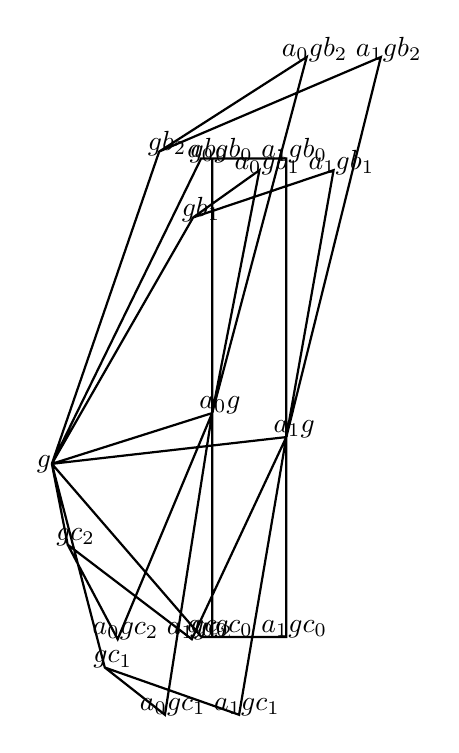
\begin{tikzpicture}
            \draw[thick](0,0)(0,0) -- (1.894562670007708,3.876197462580974) -- (2.0358015888101937,3.876197462580974) -- (2.0358015888101937,0.6444059623579539) -- (0,0)
(0,0) -- (1.7940968695318662,3.12856045647038) -- (2.6358015888101938,3.72856045647038) -- (2.0358015888101937,0.6444059623579539) -- (0,0)
(0,0) -- (1.3630927809275526,3.965570820675299) -- (3.235801588810194,5.165570820675299) -- (2.0358015888101937,0.6444059623579539) -- (0,0)
(0,0) -- (1.894562670007708,3.876197462580974) -- (2.9774212685746386,3.876197462580974) -- (2.9774212685746386,0.33952385117476724) -- (0,0)
(0,0) -- (1.7940968695318662,3.12856045647038) -- (3.5774212685746387,3.72856045647038) -- (2.9774212685746386,0.33952385117476724) -- (0,0)
(0,0) -- (1.3630927809275526,3.965570820675299) -- (4.177421268574639,5.165570820675299) -- (2.9774212685746386,0.33952385117476724) -- (0,0)
(0,0) -- (1.9011935382675718,-2.199781159406702) -- (2.0358015888101937,-2.199781159406702) -- (2.0358015888101937,0.6444059623579539) -- (0,0)
(0,0) -- (0.6723192370464812,-2.587172474217404) -- (1.4358015888101936,-3.187172474217404) -- (2.0358015888101937,0.6444059623579539) -- (0,0)
(0,0) -- (0.20098032277998623,-1.0272993300115125) -- (0.8358015888101937,-2.2272993300115127) -- (2.0358015888101937,0.6444059623579539) -- (0,0)
(0,0) -- (1.9011935382675718,-2.199781159406702) -- (2.9774212685746386,-2.199781159406702) -- (2.9774212685746386,0.33952385117476724) -- (0,0)
(0,0) -- (0.6723192370464812,-2.587172474217404) -- (2.3774212685746385,-3.187172474217404) -- (2.9774212685746386,0.33952385117476724) -- (0,0)
(0,0) -- (0.20098032277998623,-1.0272993300115125) -- (1.7774212685746387,-2.2272993300115127) -- (2.9774212685746386,0.33952385117476724) -- (0,0)
;
\node at (2.1358015888101938,3.976197462580974) {$ a_{ 0  } gb_{ 0 } $};
\node at (2.735801588810194,3.82856045647038) {$ a_{ 0  } gb_{ 1 } $};
\node at (3.335801588810194,5.265570820675299) {$ a_{ 0  } gb_{ 2 } $};
\node at (3.0774212685746387,3.976197462580974) {$ a_{ 1  } gb_{ 0 } $};
\node at (3.677421268574639,3.82856045647038) {$ a_{ 1  } gb_{ 1 } $};
\node at (4.2774212685746384,5.265570820675299) {$ a_{ 1  } gb_{ 2 } $};
\node at (2.1358015888101938,-2.0997811594067017) {$ a_{ 0  } gc_{ 0 } $};
\node at (1.5358015888101937,-3.087172474217404) {$ a_{ 0  } gc_{ 1 } $};
\node at (0.9358015888101937,-2.1272993300115126) {$ a_{ 0  } gc_{ 2 } $};
\node at (3.0774212685746387,-2.0997811594067017) {$ a_{ 1  } gc_{ 0 } $};
\node at (2.4774212685746386,-3.087172474217404) {$ a_{ 1  } gc_{ 1 } $};
\node at (1.8774212685746388,-2.1272993300115126) {$ a_{ 1  } gc_{ 2 } $};
\node at (-0.1,0) {$ g $};
\node at (2.1358015888101938,0.7444059623579539) {$ a_{ 0 }g $};
\node at (3.0774212685746387,0.4395238511747672) {$ a_{ 1 }g $};
\node at (1.9945626700077081,3.976197462580974) {$ gb_{ 0 } $};
\node at (1.8940968695318663,3.22856045647038) {$ gb_{ 1 } $};
\node at (1.4630927809275527,4.0655708206752985) {$ gb_{ 2 } $};
\node at (2.0011935382675716,-2.0997811594067017) {$ gc_{ 0 } $};
\node at (0.7723192370464812,-2.4871724742174037) {$ gc_{ 1 } $};
\node at (0.3009803227799862,-0.9272993300115125) {$ gc_{ 2 } $};

            \end{tikzpicture}
            \end{center}
            \caption{Square of the complex, with edges $(g,ag), (agb, gb) \in E_A,
            (g,gb), (agb, ag) \in E_B.$ \label{fig:square}
            }
            \end{figure}
 \begin{figure}[H]
            %\label{fig:square}
            \begin{center}
            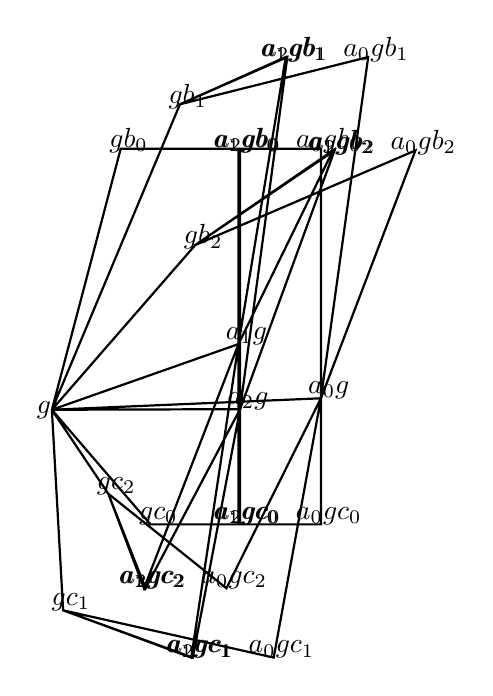
\begin{tikzpicture}
            \draw[thick](0,0)(0,0) -- (0.8741602198977303,3.3140563825118488) -- (3.417069586273492,3.3140563825118488) -- (3.417069586273492,0.14560291555199112) -- (0,0)
(0,0) -- (1.626177571045872,3.879027797073454) -- (4.017069586273492,4.479027797073454) -- (3.417069586273492,0.14560291555199112) -- (0,0)
(0,0) -- (1.8223221483435423,2.093019411617973) -- (4.617069586273492,3.2930194116179727) -- (3.417069586273492,0.14560291555199112) -- (0,0)
(0,0) -- (0.8741602198977303,3.3140563825118488) -- (2.3701477418522527,3.3140563825118488) -- (2.3701477418522527,0.8340856166454461) -- (0,0)
(0,0) -- (1.626177571045872,3.879027797073454) -- (2.970147741852253,4.479027797073454) -- (2.3701477418522527,0.8340856166454461) -- (0,0)
(0,0) -- (1.8223221483435423,2.093019411617973) -- (3.570147741852253,3.2930194116179727) -- (2.3701477418522527,0.8340856166454461) -- (0,0)
(0,0) -- (0.8741602198977303,3.3140563825118488) -- (2.390132376595972,3.3140563825118488) -- (2.390132376595972,0.007207074854495721) -- (0,0)
(0,0) -- (1.626177571045872,3.879027797073454) -- (2.990132376595972,4.479027797073454) -- (2.390132376595972,0.007207074854495721) -- (0,0)
(0,0) -- (1.8223221483435423,2.093019411617973) -- (3.590132376595972,3.2930194116179727) -- (2.390132376595972,0.007207074854495721) -- (0,0)
(0,0) -- (1.252435269783685,-1.4558934037815074) -- (3.417069586273492,-1.4558934037815074) -- (3.417069586273492,0.14560291555199112) -- (0,0)
(0,0) -- (0.1432090470076881,-2.5473184086279166) -- (2.817069586273492,-3.1473184086279167) -- (3.417069586273492,0.14560291555199112) -- (0,0)
(0,0) -- (0.7167557970943932,-1.0668626608986558) -- (2.2170695862734924,-2.2668626608986555) -- (3.417069586273492,0.14560291555199112) -- (0,0)
(0,0) -- (1.252435269783685,-1.4558934037815074) -- (2.3701477418522527,-1.4558934037815074) -- (2.3701477418522527,0.8340856166454461) -- (0,0)
(0,0) -- (0.1432090470076881,-2.5473184086279166) -- (1.7701477418522527,-3.1473184086279167) -- (2.3701477418522527,0.8340856166454461) -- (0,0)
(0,0) -- (0.7167557970943932,-1.0668626608986558) -- (1.1701477418522528,-2.2668626608986555) -- (2.3701477418522527,0.8340856166454461) -- (0,0)
(0,0) -- (1.252435269783685,-1.4558934037815074) -- (2.390132376595972,-1.4558934037815074) -- (2.390132376595972,0.007207074854495721) -- (0,0)
(0,0) -- (0.1432090470076881,-2.5473184086279166) -- (1.790132376595972,-3.1473184086279167) -- (2.390132376595972,0.007207074854495721) -- (0,0)
(0,0) -- (0.7167557970943932,-1.0668626608986558) -- (1.1901323765959722,-2.2668626608986555) -- (2.390132376595972,0.007207074854495721) -- (0,0)
;
\node at (3.517069586273492,3.414056382511849) {$ a_{ 0  } gb_{ 0 } $};
\node at (4.117069586273492,4.579027797073453) {$ a_{ 0  } gb_{ 1 } $};
\node at (4.7170695862734915,3.393019411617973) {$ a_{ 0  } gb_{ 2 } $};
\node at (2.470147741852253,3.414056382511849) {$ a_{ 1  } gb_{ 0 } $};
\node at (3.070147741852253,4.579027797073453) {$ a_{ 1  } gb_{ 1 } $};
\node at (3.670147741852253,3.393019411617973) {$ a_{ 1  } gb_{ 2 } $};
\node at (2.490132376595972,3.414056382511849) {$ a_{ 2  } gb_{ 0 } $};
\node at (3.0901323765959723,4.579027797073453) {$ a_{ 2  } gb_{ 1 } $};
\node at (3.690132376595972,3.393019411617973) {$ a_{ 2  } gb_{ 2 } $};
\node at (3.517069586273492,-1.3558934037815074) {$ a_{ 0  } gc_{ 0 } $};
\node at (2.917069586273492,-3.0473184086279166) {$ a_{ 0  } gc_{ 1 } $};
\node at (2.3170695862734925,-2.1668626608986554) {$ a_{ 0  } gc_{ 2 } $};
\node at (2.470147741852253,-1.3558934037815074) {$ a_{ 1  } gc_{ 0 } $};
\node at (1.8701477418522527,-3.0473184086279166) {$ a_{ 1  } gc_{ 1 } $};
\node at (1.2701477418522529,-2.1668626608986554) {$ a_{ 1  } gc_{ 2 } $};
\node at (2.490132376595972,-1.3558934037815074) {$ a_{ 2  } gc_{ 0 } $};
\node at (1.890132376595972,-3.0473184086279166) {$ a_{ 2  } gc_{ 1 } $};
\node at (1.2901323765959722,-2.1668626608986554) {$ a_{ 2  } gc_{ 2 } $};
\node at (-0.1,0) {$ g $};
\node at (3.517069586273492,0.24560291555199112) {$ a_{ 0 }g $};
\node at (2.470147741852253,0.9340856166454461) {$ a_{ 1 }g $};
\node at (2.490132376595972,0.10720707485449572) {$ a_{ 2 }g $};
\node at (0.9741602198977303,3.414056382511849) {$ gb_{ 0 } $};
\node at (1.726177571045872,3.979027797073454) {$ gb_{ 1 } $};
\node at (1.9223221483435424,2.193019411617973) {$ gb_{ 2 } $};
\node at (1.352435269783685,-1.3558934037815074) {$ gc_{ 0 } $};
\node at (0.2432090470076881,-2.4473184086279165) {$ gc_{ 1 } $};
\node at (0.8167557970943932,-0.9668626608986558) {$ gc_{ 2 } $};

            \end{tikzpicture}
            \end{center}
            \caption{Square of the complex, with edges $(g,ag), (agb, gb) \in E_A,
            (g,gb), (agb, ag) \in E_B.$ \label{fig:square}
            }
            \end{figure}
 \begin{figure}[H]
            %\label{fig:square}
            \begin{center}
            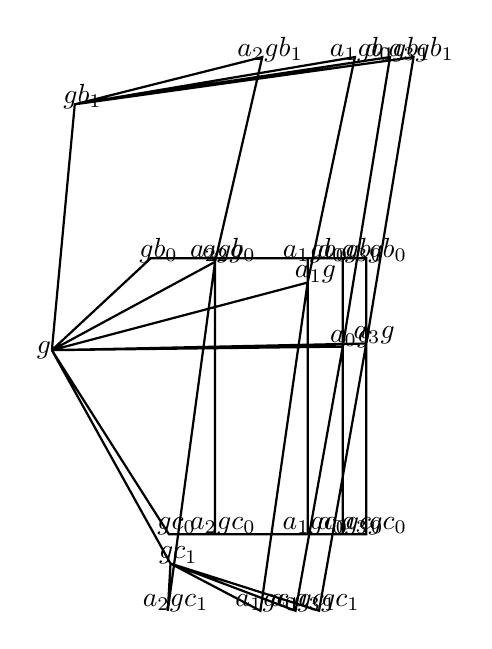
\begin{tikzpicture}
            \draw[thick](0,0)(0,0) -- (1.25623124909887,1.1676365829074817) -- (3.694297773574389,1.1676365829074817) -- (3.694297773574389,0.04499019677996996) -- (0,0)
(0,0) -- (0.2910072753139341,3.1222967129310213) -- (4.294297773574389,3.7222967129310214) -- (3.694297773574389,0.04499019677996996) -- (0,0)
(0,0) -- (1.25623124909887,1.1676365829074817) -- (3.248310272284721,1.1676365829074817) -- (3.248310272284721,0.8589193946157628) -- (0,0)
(0,0) -- (0.2910072753139341,3.1222967129310213) -- (3.848310272284721,3.7222967129310214) -- (3.248310272284721,0.8589193946157628) -- (0,0)
(0,0) -- (1.25623124909887,1.1676365829074817) -- (2.072185032233559,1.1676365829074817) -- (2.072185032233559,1.1215551999900504) -- (0,0)
(0,0) -- (0.2910072753139341,3.1222967129310213) -- (2.672185032233559,3.7222967129310214) -- (2.072185032233559,1.1215551999900504) -- (0,0)
(0,0) -- (1.25623124909887,1.1676365829074817) -- (3.99302268124919,1.1676365829074817) -- (3.99302268124919,0.08476687057170915) -- (0,0)
(0,0) -- (0.2910072753139341,3.1222967129310213) -- (4.59302268124919,3.7222967129310214) -- (3.99302268124919,0.08476687057170915) -- (0,0)
(0,0) -- (1.4858349381801887,-2.336552566741426) -- (3.694297773574389,-2.336552566741426) -- (3.694297773574389,0.04499019677996996) -- (0,0)
(0,0) -- (1.5065524265239558,-2.7100639657609285) -- (3.094297773574389,-3.3100639657609285) -- (3.694297773574389,0.04499019677996996) -- (0,0)
(0,0) -- (1.4858349381801887,-2.336552566741426) -- (3.248310272284721,-2.336552566741426) -- (3.248310272284721,0.8589193946157628) -- (0,0)
(0,0) -- (1.5065524265239558,-2.7100639657609285) -- (2.648310272284721,-3.3100639657609285) -- (3.248310272284721,0.8589193946157628) -- (0,0)
(0,0) -- (1.4858349381801887,-2.336552566741426) -- (2.072185032233559,-2.336552566741426) -- (2.072185032233559,1.1215551999900504) -- (0,0)
(0,0) -- (1.5065524265239558,-2.7100639657609285) -- (1.472185032233559,-3.3100639657609285) -- (2.072185032233559,1.1215551999900504) -- (0,0)
(0,0) -- (1.4858349381801887,-2.336552566741426) -- (3.99302268124919,-2.336552566741426) -- (3.99302268124919,0.08476687057170915) -- (0,0)
(0,0) -- (1.5065524265239558,-2.7100639657609285) -- (3.3930226812491897,-3.3100639657609285) -- (3.99302268124919,0.08476687057170915) -- (0,0)
;
\node at (3.7942977735743892,1.2676365829074818) {$ a_{ 0  } gb_{ 0 } $};
\node at (4.394297773574388,3.8222967129310215) {$ a_{ 0  } gb_{ 1 } $};
\node at (3.348310272284721,1.2676365829074818) {$ a_{ 1  } gb_{ 0 } $};
\node at (3.948310272284721,3.8222967129310215) {$ a_{ 1  } gb_{ 1 } $};
\node at (2.172185032233559,1.2676365829074818) {$ a_{ 2  } gb_{ 0 } $};
\node at (2.7721850322335593,3.8222967129310215) {$ a_{ 2  } gb_{ 1 } $};
\node at (4.09302268124919,1.2676365829074818) {$ a_{ 3  } gb_{ 0 } $};
\node at (4.6930226812491895,3.8222967129310215) {$ a_{ 3  } gb_{ 1 } $};
\node at (3.7942977735743892,-2.236552566741426) {$ a_{ 0  } gc_{ 0 } $};
\node at (3.194297773574389,-3.2100639657609285) {$ a_{ 0  } gc_{ 1 } $};
\node at (3.348310272284721,-2.236552566741426) {$ a_{ 1  } gc_{ 0 } $};
\node at (2.748310272284721,-3.2100639657609285) {$ a_{ 1  } gc_{ 1 } $};
\node at (2.172185032233559,-2.236552566741426) {$ a_{ 2  } gc_{ 0 } $};
\node at (1.572185032233559,-3.2100639657609285) {$ a_{ 2  } gc_{ 1 } $};
\node at (4.09302268124919,-2.236552566741426) {$ a_{ 3  } gc_{ 0 } $};
\node at (3.49302268124919,-3.2100639657609285) {$ a_{ 3  } gc_{ 1 } $};
\node at (-0.1,0) {$ g $};
\node at (3.7942977735743892,0.14499019677996997) {$ a_{ 0 }g $};
\node at (3.348310272284721,0.9589193946157628) {$ a_{ 1 }g $};
\node at (2.172185032233559,1.2215551999900505) {$ a_{ 2 }g $};
\node at (4.09302268124919,0.18476687057170915) {$ a_{ 3 }g $};
\node at (1.3562312490988702,1.2676365829074818) {$ gb_{ 0 } $};
\node at (0.3910072753139341,3.2222967129310214) {$ gb_{ 1 } $};
\node at (1.5858349381801888,-2.236552566741426) {$ gc_{ 0 } $};
\node at (1.606552426523956,-2.6100639657609284) {$ gc_{ 1 } $};

            \end{tikzpicture}
            \end{center}
            \caption{Square of the complex, with edges $(g,ag), (agb, gb) \in E_A,
            (g,gb), (agb, ag) \in E_B.$ \label{fig:square}
            }
            \end{figure}
 \begin{figure}[H]
            %\label{fig:square}
            \begin{center}
            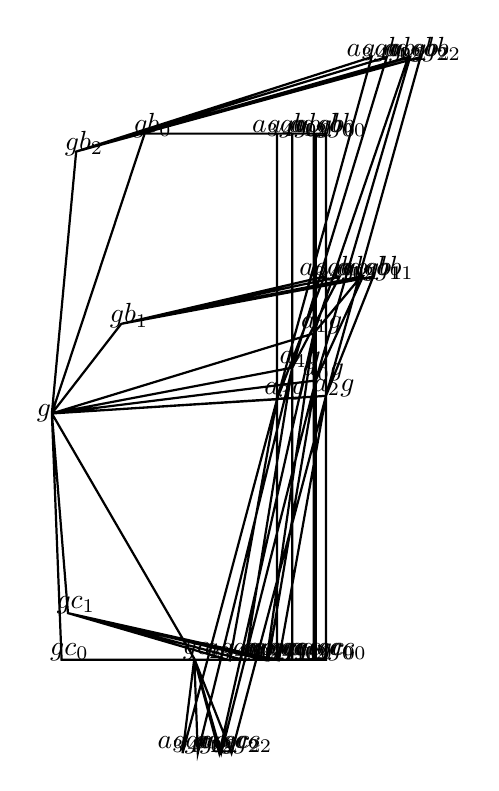
\begin{tikzpicture}
            \draw[thick](0,0)(0,0) -- (1.1780745400022778,3.5539683540917837) -- (3.3503209620477623,3.5539683540917837) -- (3.3503209620477623,0.41842364239373475) -- (0,0)
(0,0) -- (0.8813492120002457,1.1380373809373228) -- (3.9503209620477624,1.7380373809373229) -- (3.3503209620477623,0.41842364239373475) -- (0,0)
(0,0) -- (0.3088242371248713,3.3260411770860117) -- (4.5503209620477625,4.526041177086012) -- (3.3503209620477623,0.41842364239373475) -- (0,0)
(0,0) -- (1.1780745400022778,3.5539683540917837) -- (3.325858584394887,3.5539683540917837) -- (3.325858584394887,1.016480836045115) -- (0,0)
(0,0) -- (0.8813492120002457,1.1380373809373228) -- (3.925858584394887,1.7380373809373229) -- (3.325858584394887,1.016480836045115) -- (0,0)
(0,0) -- (0.3088242371248713,3.3260411770860117) -- (4.525858584394887,4.526041177086012) -- (3.325858584394887,1.016480836045115) -- (0,0)
(0,0) -- (1.1780745400022778,3.5539683540917837) -- (3.4814846414569893,3.5539683540917837) -- (3.4814846414569893,0.2234017230258627) -- (0,0)
(0,0) -- (0.8813492120002457,1.1380373809373228) -- (4.081484641456989,1.7380373809373229) -- (3.4814846414569893,0.2234017230258627) -- (0,0)
(0,0) -- (0.3088242371248713,3.3260411770860117) -- (4.681484641456989,4.526041177086012) -- (3.4814846414569893,0.2234017230258627) -- (0,0)
(0,0) -- (1.1780745400022778,3.5539683540917837) -- (2.8598024899609165,3.5539683540917837) -- (2.8598024899609165,0.18015852499585944) -- (0,0)
(0,0) -- (0.8813492120002457,1.1380373809373228) -- (3.4598024899609165,1.7380373809373229) -- (2.8598024899609165,0.18015852499585944) -- (0,0)
(0,0) -- (0.3088242371248713,3.3260411770860117) -- (4.059802489960917,4.526041177086012) -- (2.8598024899609165,0.18015852499585944) -- (0,0)
(0,0) -- (1.1780745400022778,3.5539683540917837) -- (3.05349443380494,3.5539683540917837) -- (3.05349443380494,0.581678161953079) -- (0,0)
(0,0) -- (0.8813492120002457,1.1380373809373228) -- (3.65349443380494,1.7380373809373229) -- (3.05349443380494,0.581678161953079) -- (0,0)
(0,0) -- (0.3088242371248713,3.3260411770860117) -- (4.25349443380494,4.526041177086012) -- (3.05349443380494,0.581678161953079) -- (0,0)
(0,0) -- (0.12336223828790494,-3.1288317223559443) -- (3.3503209620477623,-3.1288317223559443) -- (3.3503209620477623,0.41842364239373475) -- (0,0)
(0,0) -- (0.20423324616153393,-2.535704518058062) -- (2.750320962047762,-3.1357045180580623) -- (3.3503209620477623,0.41842364239373475) -- (0,0)
(0,0) -- (1.8087903654109072,-3.114122712204754) -- (2.150320962047762,-4.314122712204754) -- (3.3503209620477623,0.41842364239373475) -- (0,0)
(0,0) -- (0.12336223828790494,-3.1288317223559443) -- (3.325858584394887,-3.1288317223559443) -- (3.325858584394887,1.016480836045115) -- (0,0)
(0,0) -- (0.20423324616153393,-2.535704518058062) -- (2.725858584394887,-3.1357045180580623) -- (3.325858584394887,1.016480836045115) -- (0,0)
(0,0) -- (1.8087903654109072,-3.114122712204754) -- (2.125858584394887,-4.314122712204754) -- (3.325858584394887,1.016480836045115) -- (0,0)
(0,0) -- (0.12336223828790494,-3.1288317223559443) -- (3.4814846414569893,-3.1288317223559443) -- (3.4814846414569893,0.2234017230258627) -- (0,0)
(0,0) -- (0.20423324616153393,-2.535704518058062) -- (2.8814846414569892,-3.1357045180580623) -- (3.4814846414569893,0.2234017230258627) -- (0,0)
(0,0) -- (1.8087903654109072,-3.114122712204754) -- (2.2814846414569896,-4.314122712204754) -- (3.4814846414569893,0.2234017230258627) -- (0,0)
(0,0) -- (0.12336223828790494,-3.1288317223559443) -- (2.8598024899609165,-3.1288317223559443) -- (2.8598024899609165,0.18015852499585944) -- (0,0)
(0,0) -- (0.20423324616153393,-2.535704518058062) -- (2.2598024899609164,-3.1357045180580623) -- (2.8598024899609165,0.18015852499585944) -- (0,0)
(0,0) -- (1.8087903654109072,-3.114122712204754) -- (1.6598024899609165,-4.314122712204754) -- (2.8598024899609165,0.18015852499585944) -- (0,0)
(0,0) -- (0.12336223828790494,-3.1288317223559443) -- (3.05349443380494,-3.1288317223559443) -- (3.05349443380494,0.581678161953079) -- (0,0)
(0,0) -- (0.20423324616153393,-2.535704518058062) -- (2.45349443380494,-3.1357045180580623) -- (3.05349443380494,0.581678161953079) -- (0,0)
(0,0) -- (1.8087903654109072,-3.114122712204754) -- (1.8534944338049402,-4.314122712204754) -- (3.05349443380494,0.581678161953079) -- (0,0)
;
\node at (3.4503209620477624,3.6539683540917838) {$ a_{ 0  } gb_{ 0 } $};
\node at (4.0503209620477625,1.838037380937323) {$ a_{ 0  } gb_{ 1 } $};
\node at (4.650320962047762,4.6260411770860115) {$ a_{ 0  } gb_{ 2 } $};
\node at (3.425858584394887,3.6539683540917838) {$ a_{ 1  } gb_{ 0 } $};
\node at (4.025858584394887,1.838037380937323) {$ a_{ 1  } gb_{ 1 } $};
\node at (4.625858584394886,4.6260411770860115) {$ a_{ 1  } gb_{ 2 } $};
\node at (3.5814846414569894,3.6539683540917838) {$ a_{ 2  } gb_{ 0 } $};
\node at (4.181484641456989,1.838037380937323) {$ a_{ 2  } gb_{ 1 } $};
\node at (4.781484641456989,4.6260411770860115) {$ a_{ 2  } gb_{ 2 } $};
\node at (2.9598024899609165,3.6539683540917838) {$ a_{ 3  } gb_{ 0 } $};
\node at (3.5598024899609166,1.838037380937323) {$ a_{ 3  } gb_{ 1 } $};
\node at (4.159802489960916,4.6260411770860115) {$ a_{ 3  } gb_{ 2 } $};
\node at (3.15349443380494,3.6539683540917838) {$ a_{ 4  } gb_{ 0 } $};
\node at (3.7534944338049403,1.838037380937323) {$ a_{ 4  } gb_{ 1 } $};
\node at (4.35349443380494,4.6260411770860115) {$ a_{ 4  } gb_{ 2 } $};
\node at (3.4503209620477624,-3.0288317223559442) {$ a_{ 0  } gc_{ 0 } $};
\node at (2.8503209620477623,-3.035704518058062) {$ a_{ 0  } gc_{ 1 } $};
\node at (2.250320962047762,-4.214122712204754) {$ a_{ 0  } gc_{ 2 } $};
\node at (3.425858584394887,-3.0288317223559442) {$ a_{ 1  } gc_{ 0 } $};
\node at (2.825858584394887,-3.035704518058062) {$ a_{ 1  } gc_{ 1 } $};
\node at (2.2258585843948873,-4.214122712204754) {$ a_{ 1  } gc_{ 2 } $};
\node at (3.5814846414569894,-3.0288317223559442) {$ a_{ 2  } gc_{ 0 } $};
\node at (2.9814846414569893,-3.035704518058062) {$ a_{ 2  } gc_{ 1 } $};
\node at (2.3814846414569897,-4.214122712204754) {$ a_{ 2  } gc_{ 2 } $};
\node at (2.9598024899609165,-3.0288317223559442) {$ a_{ 3  } gc_{ 0 } $};
\node at (2.3598024899609165,-3.035704518058062) {$ a_{ 3  } gc_{ 1 } $};
\node at (1.7598024899609166,-4.214122712204754) {$ a_{ 3  } gc_{ 2 } $};
\node at (3.15349443380494,-3.0288317223559442) {$ a_{ 4  } gc_{ 0 } $};
\node at (2.55349443380494,-3.035704518058062) {$ a_{ 4  } gc_{ 1 } $};
\node at (1.9534944338049403,-4.214122712204754) {$ a_{ 4  } gc_{ 2 } $};
\node at (-0.1,0) {$ g $};
\node at (3.4503209620477624,0.5184236423937347) {$ a_{ 0 }g $};
\node at (3.425858584394887,1.116480836045115) {$ a_{ 1 }g $};
\node at (3.5814846414569894,0.3234017230258627) {$ a_{ 2 }g $};
\node at (2.9598024899609165,0.28015852499585947) {$ a_{ 3 }g $};
\node at (3.15349443380494,0.681678161953079) {$ a_{ 4 }g $};
\node at (1.278074540002278,3.6539683540917838) {$ gb_{ 0 } $};
\node at (0.9813492120002457,1.2380373809373229) {$ gb_{ 1 } $};
\node at (0.40882423712487126,3.4260411770860117) {$ gb_{ 2 } $};
\node at (0.22336223828790494,-3.0288317223559442) {$ gc_{ 0 } $};
\node at (0.3042332461615339,-2.435704518058062) {$ gc_{ 1 } $};
\node at (1.9087903654109073,-3.014122712204754) {$ gc_{ 2 } $};

            \end{tikzpicture}
            \end{center}
            \caption{Square of the complex, with edges $(g,ag), (agb, gb) \in E_A,
            (g,gb), (agb, ag) \in E_B.$ \label{fig:square}
            }
            \end{figure}
 \begin{figure}[H]
            %\label{fig:square}
            \begin{center}
            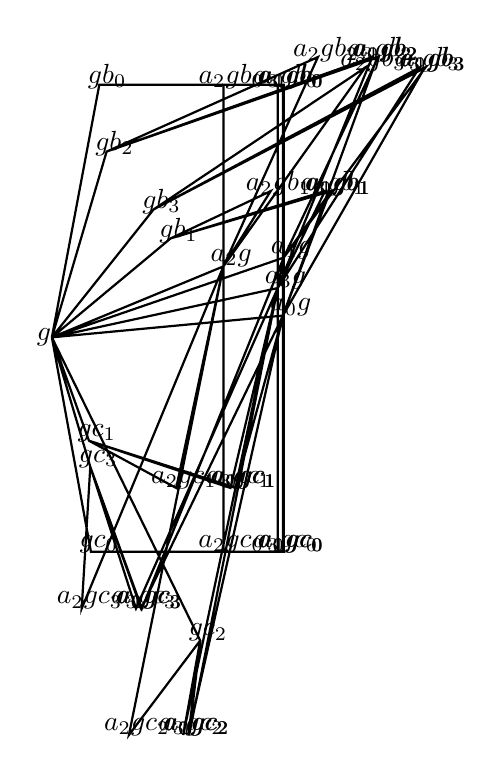
\begin{tikzpicture}
            \draw[thick](0,0)(0,0) -- (0.6026852948185268,3.2086385726996323) -- (2.933954865035155,3.2086385726996323) -- (2.933954865035155,0.2761310065150937) -- (0,0)
(0,0) -- (1.5094624415691404,1.256962763897579) -- (3.533954865035155,1.8569627638975792) -- (2.933954865035155,0.2761310065150937) -- (0,0)
(0,0) -- (0.6955363174275835,2.359392767486125) -- (4.133954865035155,3.559392767486125) -- (2.933954865035155,0.2761310065150937) -- (0,0)
(0,0) -- (1.2934380469502926,1.6255694077421128) -- (4.733954865035155,3.4255694077421124) -- (2.933954865035155,0.2761310065150937) -- (0,0)
(0,0) -- (0.6026852948185268,3.2086385726996323) -- (2.943650836623738,3.2086385726996323) -- (2.943650836623738,1.0120757136468275) -- (0,0)
(0,0) -- (1.5094624415691404,1.256962763897579) -- (3.5436508366237383,1.8569627638975792) -- (2.943650836623738,1.0120757136468275) -- (0,0)
(0,0) -- (0.6955363174275835,2.359392767486125) -- (4.143650836623738,3.559392767486125) -- (2.943650836623738,1.0120757136468275) -- (0,0)
(0,0) -- (1.2934380469502926,1.6255694077421128) -- (4.743650836623738,3.4255694077421124) -- (2.943650836623738,1.0120757136468275) -- (0,0)
(0,0) -- (0.6026852948185268,3.2086385726996323) -- (2.1787861782480475,3.2086385726996323) -- (2.1787861782480475,0.9013036317386671) -- (0,0)
(0,0) -- (1.5094624415691404,1.256962763897579) -- (2.7787861782480476,1.8569627638975792) -- (2.1787861782480475,0.9013036317386671) -- (0,0)
(0,0) -- (0.6955363174275835,2.359392767486125) -- (3.3787861782480473,3.559392767486125) -- (2.1787861782480475,0.9013036317386671) -- (0,0)
(0,0) -- (1.2934380469502926,1.6255694077421128) -- (3.9787861782480474,3.4255694077421124) -- (2.1787861782480475,0.9013036317386671) -- (0,0)
(0,0) -- (0.6026852948185268,3.2086385726996323) -- (2.8680424364237003,3.2086385726996323) -- (2.8680424364237003,0.6257497168249186) -- (0,0)
(0,0) -- (1.5094624415691404,1.256962763897579) -- (3.4680424364237004,1.8569627638975792) -- (2.8680424364237003,0.6257497168249186) -- (0,0)
(0,0) -- (0.6955363174275835,2.359392767486125) -- (4.0680424364237,3.559392767486125) -- (2.8680424364237003,0.6257497168249186) -- (0,0)
(0,0) -- (1.2934380469502926,1.6255694077421128) -- (4.6680424364237005,3.4255694077421124) -- (2.8680424364237003,0.6257497168249186) -- (0,0)
(0,0) -- (0.4962517896528358,-2.724151759111148) -- (2.933954865035155,-2.724151759111148) -- (2.933954865035155,0.2761310065150937) -- (0,0)
(0,0) -- (0.47095355687713303,-1.312883845717891) -- (2.333954865035155,-1.9128838457178912) -- (2.933954865035155,0.2761310065150937) -- (0,0)
(0,0) -- (1.8839458216893044,-3.85009935639023) -- (1.733954865035155,-5.05009935639023) -- (2.933954865035155,0.2761310065150937) -- (0,0)
(0,0) -- (0.4881337182912988,-1.6439307096864808) -- (1.1339548650351552,-3.4439307096864806) -- (2.933954865035155,0.2761310065150937) -- (0,0)
(0,0) -- (0.4962517896528358,-2.724151759111148) -- (2.943650836623738,-2.724151759111148) -- (2.943650836623738,1.0120757136468275) -- (0,0)
(0,0) -- (0.47095355687713303,-1.312883845717891) -- (2.343650836623738,-1.9128838457178912) -- (2.943650836623738,1.0120757136468275) -- (0,0)
(0,0) -- (1.8839458216893044,-3.85009935639023) -- (1.7436508366237382,-5.05009935639023) -- (2.943650836623738,1.0120757136468275) -- (0,0)
(0,0) -- (0.4881337182912988,-1.6439307096864808) -- (1.1436508366237383,-3.4439307096864806) -- (2.943650836623738,1.0120757136468275) -- (0,0)
(0,0) -- (0.4962517896528358,-2.724151759111148) -- (2.1787861782480475,-2.724151759111148) -- (2.1787861782480475,0.9013036317386671) -- (0,0)
(0,0) -- (0.47095355687713303,-1.312883845717891) -- (1.5787861782480475,-1.9128838457178912) -- (2.1787861782480475,0.9013036317386671) -- (0,0)
(0,0) -- (1.8839458216893044,-3.85009935639023) -- (0.9787861782480476,-5.05009935639023) -- (2.1787861782480475,0.9013036317386671) -- (0,0)
(0,0) -- (0.4881337182912988,-1.6439307096864808) -- (0.3787861782480477,-3.4439307096864806) -- (2.1787861782480475,0.9013036317386671) -- (0,0)
(0,0) -- (0.4962517896528358,-2.724151759111148) -- (2.8680424364237003,-2.724151759111148) -- (2.8680424364237003,0.6257497168249186) -- (0,0)
(0,0) -- (0.47095355687713303,-1.312883845717891) -- (2.2680424364237,-1.9128838457178912) -- (2.8680424364237003,0.6257497168249186) -- (0,0)
(0,0) -- (1.8839458216893044,-3.85009935639023) -- (1.6680424364237003,-5.05009935639023) -- (2.8680424364237003,0.6257497168249186) -- (0,0)
(0,0) -- (0.4881337182912988,-1.6439307096864808) -- (1.0680424364237004,-3.4439307096864806) -- (2.8680424364237003,0.6257497168249186) -- (0,0)
;
\node at (3.033954865035155,3.3086385726996324) {$ a_{ 0  } gb_{ 0 } $};
\node at (3.633954865035155,1.9569627638975793) {$ a_{ 0  } gb_{ 1 } $};
\node at (4.233954865035154,3.6593927674861253) {$ a_{ 0  } gb_{ 2 } $};
\node at (4.833954865035155,3.5255694077421125) {$ a_{ 0  } gb_{ 3 } $};
\node at (3.0436508366237383,3.3086385726996324) {$ a_{ 1  } gb_{ 0 } $};
\node at (3.6436508366237383,1.9569627638975793) {$ a_{ 1  } gb_{ 1 } $};
\node at (4.243650836623738,3.6593927674861253) {$ a_{ 1  } gb_{ 2 } $};
\node at (4.843650836623738,3.5255694077421125) {$ a_{ 1  } gb_{ 3 } $};
\node at (2.2787861782480476,3.3086385726996324) {$ a_{ 2  } gb_{ 0 } $};
\node at (2.8787861782480477,1.9569627638975793) {$ a_{ 2  } gb_{ 1 } $};
\node at (3.4787861782480474,3.6593927674861253) {$ a_{ 2  } gb_{ 2 } $};
\node at (4.0787861782480475,3.5255694077421125) {$ a_{ 2  } gb_{ 3 } $};
\node at (2.9680424364237004,3.3086385726996324) {$ a_{ 3  } gb_{ 0 } $};
\node at (3.5680424364237004,1.9569627638975793) {$ a_{ 3  } gb_{ 1 } $};
\node at (4.1680424364237,3.6593927674861253) {$ a_{ 3  } gb_{ 2 } $};
\node at (4.7680424364237,3.5255694077421125) {$ a_{ 3  } gb_{ 3 } $};
\node at (3.033954865035155,-2.624151759111148) {$ a_{ 0  } gc_{ 0 } $};
\node at (2.433954865035155,-1.812883845717891) {$ a_{ 0  } gc_{ 1 } $};
\node at (1.8339548650351551,-4.95009935639023) {$ a_{ 0  } gc_{ 2 } $};
\node at (1.2339548650351553,-3.3439307096864805) {$ a_{ 0  } gc_{ 3 } $};
\node at (3.0436508366237383,-2.624151759111148) {$ a_{ 1  } gc_{ 0 } $};
\node at (2.443650836623738,-1.812883845717891) {$ a_{ 1  } gc_{ 1 } $};
\node at (1.8436508366237383,-4.95009935639023) {$ a_{ 1  } gc_{ 2 } $};
\node at (1.2436508366237384,-3.3439307096864805) {$ a_{ 1  } gc_{ 3 } $};
\node at (2.2787861782480476,-2.624151759111148) {$ a_{ 2  } gc_{ 0 } $};
\node at (1.6787861782480475,-1.812883845717891) {$ a_{ 2  } gc_{ 1 } $};
\node at (1.0787861782480477,-4.95009935639023) {$ a_{ 2  } gc_{ 2 } $};
\node at (0.4787861782480477,-3.3439307096864805) {$ a_{ 2  } gc_{ 3 } $};
\node at (2.9680424364237004,-2.624151759111148) {$ a_{ 3  } gc_{ 0 } $};
\node at (2.3680424364237003,-1.812883845717891) {$ a_{ 3  } gc_{ 1 } $};
\node at (1.7680424364237004,-4.95009935639023) {$ a_{ 3  } gc_{ 2 } $};
\node at (1.1680424364237005,-3.3439307096864805) {$ a_{ 3  } gc_{ 3 } $};
\node at (-0.1,0) {$ g $};
\node at (3.033954865035155,0.3761310065150937) {$ a_{ 0 }g $};
\node at (3.0436508366237383,1.1120757136468276) {$ a_{ 1 }g $};
\node at (2.2787861782480476,1.0013036317386672) {$ a_{ 2 }g $};
\node at (2.9680424364237004,0.7257497168249186) {$ a_{ 3 }g $};
\node at (0.7026852948185268,3.3086385726996324) {$ gb_{ 0 } $};
\node at (1.6094624415691405,1.3569627638975792) {$ gb_{ 1 } $};
\node at (0.7955363174275835,2.459392767486125) {$ gb_{ 2 } $};
\node at (1.3934380469502927,1.7255694077421129) {$ gb_{ 3 } $};
\node at (0.5962517896528358,-2.624151759111148) {$ gc_{ 0 } $};
\node at (0.570953556877133,-1.212883845717891) {$ gc_{ 1 } $};
\node at (1.9839458216893044,-3.75009935639023) {$ gc_{ 2 } $};
\node at (0.5881337182912988,-1.5439307096864807) {$ gc_{ 3 } $};

            \end{tikzpicture}
            \end{center}
            \caption{Square of the complex, with edges $(g,ag), (agb, gb) \in E_A,
            (g,gb), (agb, ag) \in E_B.$ \label{fig:square}
            }
            \end{figure}
 
\end{multicols*}
  % \printbibliography 
\end{document}

 